\documentclass[11pt]{article}

%%%%%%%% CREATE DOCUMENT STRUCTURE %%%%%%%%
%% Language and font encodings
\usepackage[spanish]{babel}
\usepackage[utf8x]{inputenc}
\usepackage[T1]{fontenc}
%\usepackage{subfig}

%% Sets page size and margins
\usepackage[a4paper,top=3cm,bottom=2cm,left=2cm,right=2cm,marginparwidth=1.75cm]{geometry}

%% Useful packages
\usepackage{amsmath}
\usepackage{graphicx}
\usepackage[colorinlistoftodos]{todonotes}
\usepackage[colorlinks=true, allcolors=blue]{hyperref}
\usepackage{caption}
\usepackage{subcaption}
\usepackage{sectsty}
\usepackage{apacite}
\usepackage{float}
\usepackage{titling} 
\usepackage{blindtext}
\usepackage[square,sort,comma,numbers]{natbib}
\usepackage[colorinlistoftodos]{todonotes}
\usepackage{xcolor}
\definecolor{darkgreen}{rgb}{0.0, 0.4, 0.0}
\usepackage{listings}
\usepackage{color}
\usepackage{fancyhdr}

\pagestyle{fancy}
\fancyhf{}
\fancyhead[LE,RO]{IPS 2022}
\fancyhead[RE,LO]{Instalación y Reemplazo de Componentes Internos}
\fancyfoot[CE,CO]{\nouppercase\leftmark}
\fancyfoot[LE,RO]{\thepage}

\renewcommand{\headrulewidth}{2pt}
\renewcommand{\footrulewidth}{1pt}
\definecolor{dkgreen}{rgb}{0,0.6,0}
\definecolor{gray}{rgb}{0.5,0.5,0.5}
\definecolor{mauve}{rgb}{0.58,0,0.82}

\usepackage{caption}
\usepackage[newfloat]{minted}
\captionsetup[listing]{position=top}


\newcommand{\subsubsubsection}[1]{\paragraph{#1}\mbox{}\\}
\setcounter{secnumdepth}{4}
\setcounter{tocdepth}{4}
\usepackage{xpatch}
\usepackage{booktabs}

\makeatletter
\AtBeginEnvironment{minted}{\dontdofcolorbox}
\def\dontdofcolorbox{\renewcommand\fcolorbox[4][]{##4}}
\xpatchcmd{\inputminted}{\minted@fvset}{\minted@fvset\dontdofcolorbox}{}{}
\xpatchcmd{\mintinline}{\minted@fvset}{\minted@fvset\dontdofcolorbox}{}{}
\makeatother

%%%%%%%% DOCUMENT %%%%%%%%
\begin{document}
\begin{large}
%%%% Title Page
\begin{titlepage}

\newcommand{\HRule}{\rule{\linewidth}{0.5mm}} 							% horizontal line and its thickness
\noindent\begin{minipage}{0.3\textwidth}% adapt widths of minipages to your needs

\includegraphics[scale=0.5]{img/Titulo/unr.png}
\end{minipage}%
\hfill%
\begin{minipage}{0.6\textwidth}\raggedleft

\includegraphics[scale=0.25]{img/Titulo/Logo IPS upscaled.png}
\end{minipage}

\vspace{5mm}

\hline

\vspace{7.5mm}

\center 
 
% University
\textsc{\LARGE Instituto Politécnico Superior "General San Martín"}\\[1cm]

% Document info
\textsc{\Large Instalación y Reemplazo de Componentes Internos}\\[0.2cm]				
\vspace{7.5mm}

\HRule \\[0.8cm]
{ \huge \bfseries Práctica 1 MIPS (Cuestiones)}\\[0.7cm]								% Assignment
\HRule \\[2cm]
\large
\emph{Autor:}\\
Juan Ignacio Bertoni\\[1.5cm]	
\emph{Curso:}\\
6to Año Informática\\[1.5cm]	
\emph{Docente:}\\
Alejandro Rodriguez Costello\\[1.5cm]	

% Author info
{\large \today}\\[5cm]
\vfill 
\end{titlepage}



\vfill

\begin{flushleft}

\section*{Declaración de palabras en memoria}
\subsection*{Cuestion 1.1}
Podemos apreciar los valores declarados en el programa representados en el panel de datos:

\begin{figure}[H]
    \centering
    \fbox{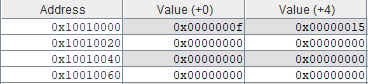
\includegraphics[scale=1]{img/proy/datos1.PNG}}
    \caption{Panel de datos}
    \label{fig:my_label}
\end{figure}

Como se puede apreciar, el valor 0x0000000f fue guardado en la dirección de memoria 0x10010000. Por otro lado, el valor 0x00000015 fue guardado en la dirección 0x10010004 -es decir, que una \textbf{palabra} o \textbf{word} distancia a cada uno de estos datos-. Ya vimos que una palabra en la arquitectura del ensamblador MIPS es un conjunto de \textit{4 bytes}. El primer valor de la tabla corresponde al 15 decimal pasado a hexadecimal, mientras que el segundo valor es el 15 en hexadecimal.



\subsection*{Cuestion 1.2}
Los valores se almacenaron en direcciones que distan de \textbf{1 palabra}, es decir, 4 bytes de memoria. Esto se debe a a la arquitectura de MIPS.

\subsection*{Cuestion 1.3}
Las etiquetas \textbf{palabra1} y \textbf{palabra2} se convierten en la respectiva dirección de memoria a la cual referenciaban sus datos. Así, palabra1 toma el valor 0x10010000, mientras que palabra2 toma el valor de 0x10010004.


\subsection*{Cuestion 1.4}
A simple vista, no parece que haya habido ninguna diferencia respecto al retorno del programa anterior. Se puede apreciar que a través de la directiva \textbf{.data}, esta vez le estamos especificando de donde empezar. En este caso, empezamos en el mismo lugar de antes (0x10010000). Luego, guardamos ambos valores en la etiqueta \textbf{palabras}. Sin embargo, en el programa ambos valores siguen viendose como valores separados, distanciados por 1 palabra.

\subsection*{Cuestion 1.5}
A continuación se muestra el código solicitado:
\begin{listing}[h]
\begin{minted}[linenos,frame=single]{nasm}
.data 0x10000000 # comienza zona de datos en la direccion dada
vector: .word 0x10, 30, 0x34, 0x20, 60 # se guardan los valores en vector
\end{minted}
\end{listing}

Para ver la tabla de valores, tenemos que dirigirnos hacia la sección \textbf{.extern}, donde se halla el conjunto de direcciones de memoria que utilizamos para el programa. Una vez allí, podemos apreciar que los valores se guardaron correctamente en hexadecimal, y los valores decimales fueron convertidos a hexa (30 a 1e y 60 a 3c).

\begin{figure}[H]
    \centering
    \fbox{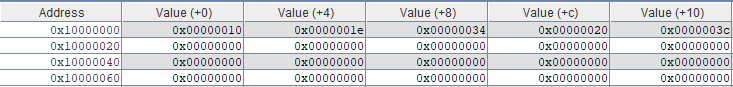
\includegraphics[scale=0.85]{img/proy/datos2.PNG}}
    \caption{Panel de datos. Como curiosidad, el \textit{offset} luego del +8 pasa a ser +c (en lugar de +12) y el +16 pasa a +10. Estas son sus conversiones a hexadecimal.}
    \label{fig:my_label}
\end{figure}




\subsection*{Cuestion 1.6}
Al intentar hacer empezar el espacio de datos en 0x10000002 con, por ejemplo, el vector 15,0x15 lo que realmente ocurre es esto:

\begin{figure}[H]
    \centering
    \fbox{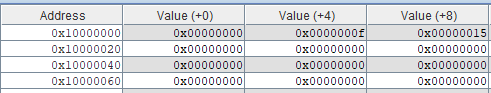
\includegraphics[scale=0.85]{img/proy/datos3.PNG}}
    \caption{Panel de datos.}
    \label{fig:my_label}
\end{figure}

Podemos observar que nuestro vector NO empezó en la dirección que le especificamos, sino que se dirigió a la \textit{dirección múltiplo de 4 más cercana}. Esto se debe a conceptos fundamentales de la arquitectura del assembler MIPS, donde los conjuntos de datos idealmente deben estar \textbf{alineados}. Esto es, colocados en porciones de datos equidistantes (en este caso, la unidad de medida son las palabras). Para que los datos estén alineados, las palabras siempre deben empezar en una dirección múltiplo de 4.

\section*{Declaración de bytes en memoria}

\subsection*{Cuestion 1.7}
La dirección de memoria que fue inicializada con el contenido especificado (0x10) fue la dirección 0x10010000.

\subsection*{Cuestion 1.8}
El valor almacenado es el 10 hexadecimal (0x10).

\subsection*{Cuestion 1.9}
Los valores almacenados en memoria se muestran a continuación:

\begin{figure}[H]
    \centering
    \fbox{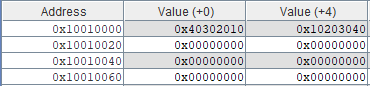
\includegraphics[scale=1]{img/proy/datos4.PNG}}
    \caption{Panel de datos.}
    \label{fig:my_label}
\end{figure}


\subsection*{Cuestion 1.10}
El simulador utiliza el tipo de alineamiento de datos \textbf{Little-endian} o "de pequeño final", en donde el valor menos significativo en la secuencia de datos (en nuestro caso, el vector \textit{palabra1}) es almacenado primero. Así, podemos observar que el vector \textbf{palabra1} compuesto por 0x10,0x20,0x30,0x40 fue guardado en forma de \textit{byte} colocando primero el valor 0x10, luego el 0x20 y terminando en 0x40 pues es el primer valor que especificamos; así se terminó formando el valor hexa 0x40302010, localizado en la dirección 0x10010000. También podemos ver que la palabra 0x10203040 fue guardada en la dirección 0x10010004.



\subsection*{Cuestion 1.11}
La etiqueta palabra1 tomó el valor de la dirección 0x10010000. Por otra parte, la etiqueta palabra2 tomó el valor de la dirección contigua 0x10010004.

\section*{Declaración de cadenas de caracteres}

\subsection*{Cuestion 1.12}
Los valores retornados al programa propuesto son los siguientes:

\begin{figure}[H]
    \centering
    \fbox{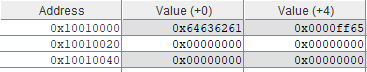
\includegraphics[scale=1]{img/proy/datos5.PNG}}
    \caption{Panel de datos.}
    \label{fig:my_label}
\end{figure}

Podemos apreciar que la salida es un conjunto de bytes amontonados en la palabra de dirección 0x10010000. Recordando que el compilador se basa en la alineación \textbf{Little endian} podríamos pensar dicho número hexadecimal como el siguiente vector: 0x61, 0x62, 0x63, 0x64. Al pasar dichos valores a decimal obtenemos respectivamente los valores: 97, 98, 99, 100. Luego, si echamos un vistazo a la tabla ascii, comprobaremos que son los caracteres respectivamente correspondientes a: 'a', 'b, 'c', 'd'. Pero recordemos que el tamaño de nuestras palabras en MIPS se reduce a 4 bytes, por lo cual nuestra letra 'e' se vio de alguna manera "truncada" hacia la siguiente palabra en memoria. En efecto, nuestra letra 'e' (\textbf{ascii 101}) se combinó en la dirección 0x10010004 junto con nuestro byte etiquetado "octeto", cuyo valor es 0xff. Así, dicha dirección guarda el arreglo constituido por los valores: 0x65, 0xff.


\subsection*{Cuestion 1.13}
Esta vez, podemos apreciar que en la dirección 0x10010004 se ha guardado un valor adicional al arreglo: 0x00. Resultando así el hexadecimal 0x00ff0065, el cual constituye los valores 0x65, 0x00, 0xff. Podemos apreciar que a nuestro string declarado se le agregó dicho caracter al final. Investigando un poco, descubrí que este 0x00 es el \textbf{terminador nulo} que ya se ha visto en lenguajes de más alto nivel como C.

\subsection*{Cuestion 1.14}
Para conseguir el mismo resultado que en el anterior problema, pero reemeplazando la directiva .ascii por .byte, no podremos declarar cadenas explícitas encerradas por comillas, sino que deberemos guardar cada caracter por separado. El código quedaría así:

\begin{listing}[h]
\begin{minted}[linenos,frame=single]{nasm}
.data
cadena: .byte 'a','b','c','d','d'
octeto: .byte 0xff
\end{minted}
\end{listing}

\section*{Reserva de espacio en memoria}

\subsection*{Cuestion 1.15}
El rango de posiciones de memoria que se ha reservado para la variable \textit{espacio} es desde 0x10010004 hasta 0x10010008. 

\subsection*{Cuestion 1.16}
En total se han reservado \textbf{2 palabras} y, recordando que 1 palabra = 4 bytes, se han reservado \textbf{8 bytes}. Por lo cual la sintaxis del compilador de MIPS es: \texttt{.space < cantidad de bytes a reservar>}.


\section*{Alineación de datos en memoria}

\subsection*{Cuestion 1.17}
El rango de posiciones de memoria que se ha reservado para la variable \textbf{espacio} esta vez fue desde 0x10010001 hasta 0x10010004. Esta vez, al haberse utilizado la directiva \texttt{.byte} en lugar de \texttt{.word}, podemos observar que el valor guardado en la dirección 0x10010004 parecería ser 0x2000, sin embargo es el valor 0x20, con un byte reservado (los otros 3 están presentes en la anterior dirección, 0x10010000).

\subsection*{Cuestion 1.18}
Estos 4 bytes reservados NO podrían constituir los bytes de una palabra, pues algunos de ellos se encuentran en palabras distintas, y recordemos que uno de los principios fundamentales de la arquitectura MIPS es la \textbf{alineación} de los segmentos de datos.

\subsection*{Cuestion 1.19}
La etiqueta byte1 se inicializó desde la dirección 0x10010000, mientras que la etiqueta byte2 -teniendo en cuenta el espacio reservado- se inicializó desde 0x10010005.

\subsection*{Cuestion 1.20}
La dirección de la etiqueta palabra se inicializó en la dirección 0x10010008, pues al ser palabra declarada bajo la directiva \textbf{.word} hay que recordar que toda palabra siempre empieza en una dirección \textit{múltiplo de 4}.

\subsection*{Cuestion 1.21}
El rango de posiciones reservado para la variable \textbf{espacio} es desde 0x10010004 hasta 0x10010007.

\subsection*{Cuestion 1.22}
Lo que la directiva \textbf{.align} hizo fue alinear el siguiente dato (en nuestro caso el byte 0x20) a una dirección de memoria múltiplo de $2^n$, siendo $n=2$ en nuestro caso. Por lo cual, al ser $2^2=4$ entonces el siguiente dato fue alineado a un múltiplo de 4, siendo así completamente adecuandos los 4 bytes reservados por la variable \textbf{espacio} para constituir una palabra, pues están alineados.





\end{flushleft}
\end{large}

\end{document}